\chapter{Konzept}
\label{chap:konzept}

\section{Beschaffung und Zulieferung}
\subsection{Datenübermittlungskonzept}
\subsection{Echtzeitauslieferung}
\subsection{Caching}

\section{Verarbeitung}
\subsection{}

\section{Anordnung und Zuweisung}

\subsection{Diagrammanordnungsverfahren}
\label{subsec:diagrammanordnungsverfahren}
Das Diagrammanordnungsverfahren beschreibt den Prozess, einzelne Diagramme in einem Dashboard anzuordnen.
Um das Verfahren zu vereinfachen, ist ein automatisches Anordnen der Diagramme diagonal sowie vertikal vorgesehen.
Die Anordnung der einzelnen Diagramme soll mithilfe der FlexBox Technologie implementiert werden.
\footnote{CSS Flexible Box Layout, bekannt als FlexBox, ist ein standardisiertes Anordnungsmuster, das von allen gängigen Browsern unterstützt wird.\cite{CanIUseFlexBox}}
Im mobilen Format sollen die einzelnen Diagramme untereinander aufgelistet werden. 

\begin{figure}
    \begin{center}
    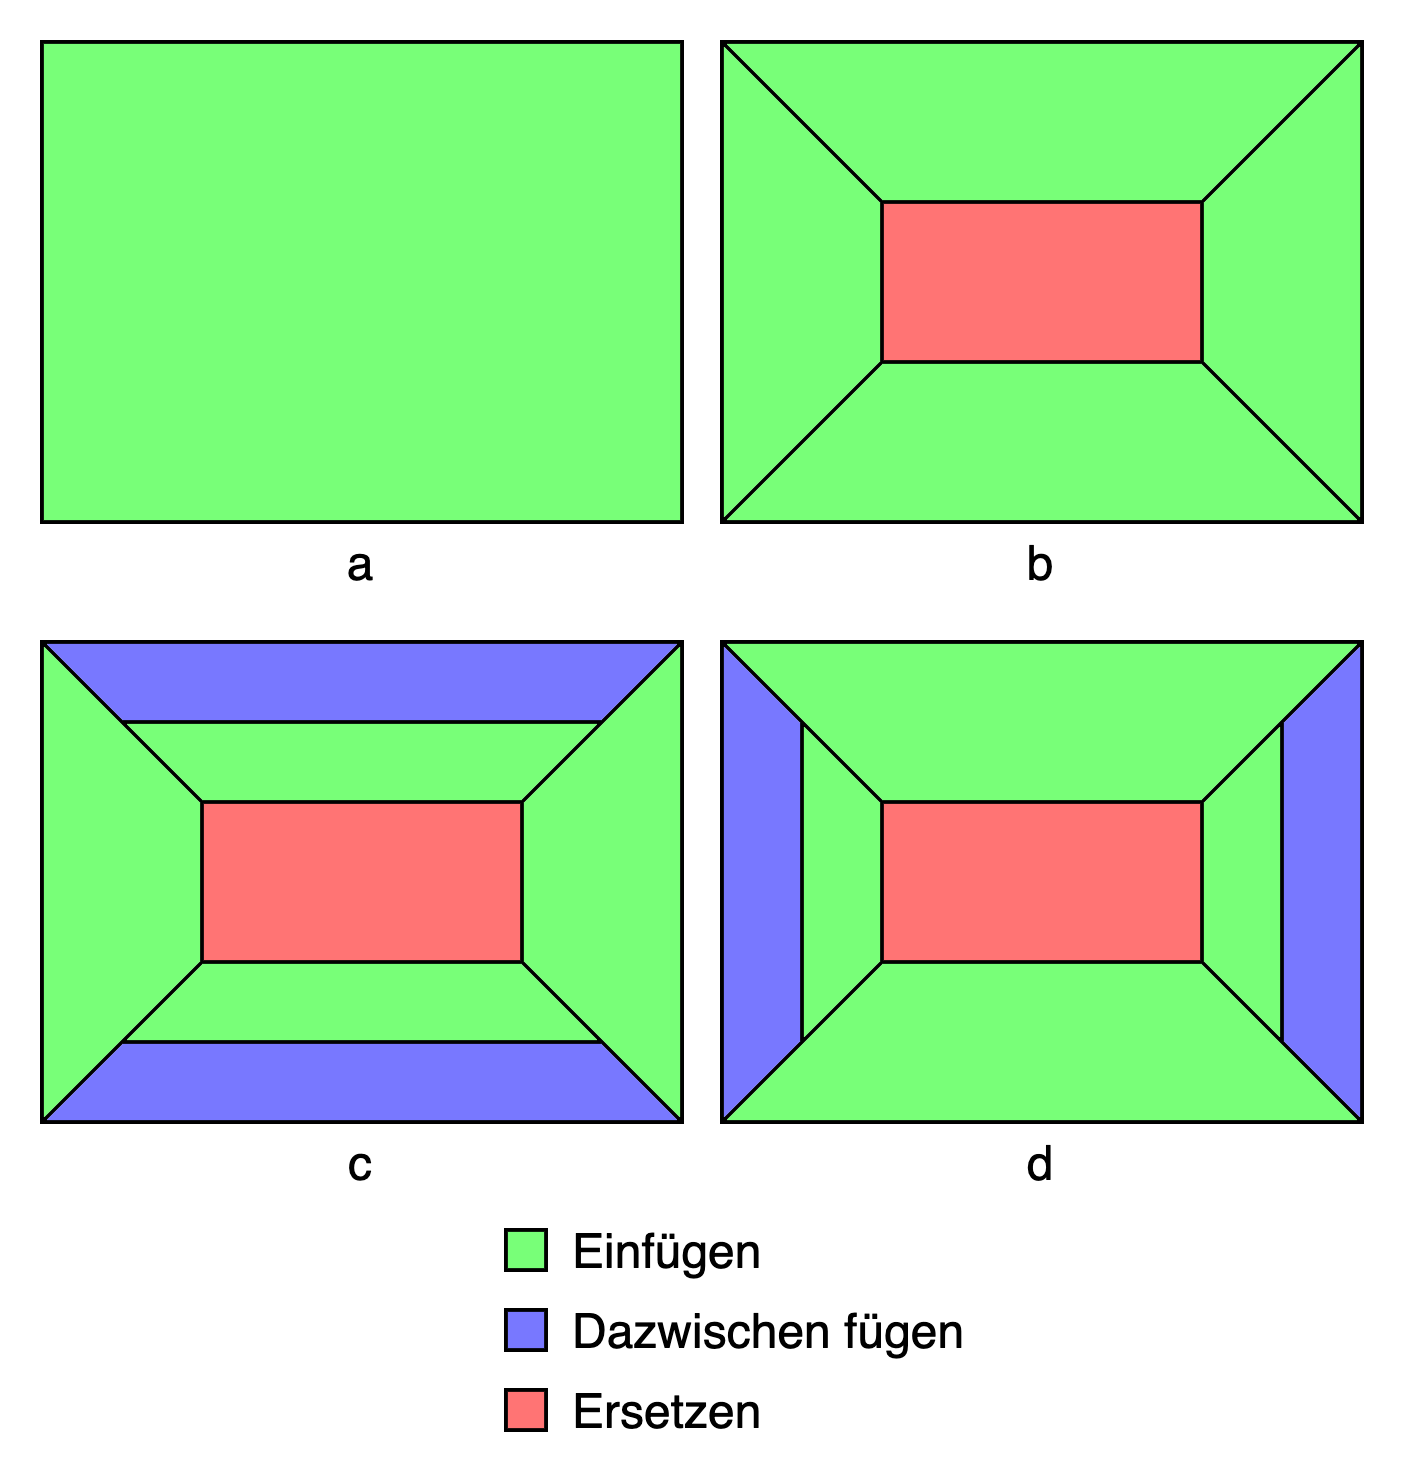
\includegraphics[scale=0.2]{img/abbildungen/DiagrammanordnungsverfahrenMitLegende}
    \end{center}
    \caption{Diagrammanordnunsverfahren}
    \label{figure:diagrammanordnungabbildung}
\end{figure}

Die Diagramme sollen nach und nach per Drag and Drop in das Dashboard integriert werden. Dieses Verfahren
wird in Abbildung \ref{figure:diagrammanordnungabbildung} dargestellt. \(a\) beschreibt den
initialen Zustand eines leeren Dashboards. Hier kann man durch Drag and Drop das erste Diagramm dem Dashboard
zuordnen. \(b\) beschreibt den Zustand des Dashboards mit genau einem enthaltenen Diagramm. Hier kann man das
neue Diagramm in alle Richtungen einfügen. Dabei Teilt das bestehende Diagram den Platz mit dem neuen gleichmäßig
auf. Bei der mittigen Positionierung wird das vorhandene Diagramm durch das neue ersetzt. \(c\) und \(d\)
beschreiben den Zustand, bei dem sich mehr als ein Diagramm im Dashboard befindet. Wenn man im Zustand \(b\)
ein Diagramm oberhalb oder unterhalb einfügt, bilden die beiden Diagramme eine Spalte. Beide dieser Diagramme
beinhalten nun den Zustand \(c\). Additional zu den möglichkeiten von Zustand \(b\), kann hier ein Diagramm
auch dazwischen gefügt werden. Es teilt sich dann den Platz mit den anderen Diagrammen in der Spalte.
Fügt man bei Zustand \(b\) ein Diagramm links oder rechts ein, bilden die beiden Diagramme eine Reihe.
Beide dieser Diagramme befinden sich nun in Zustand \(d\). Additional zu Zustand \(b\) können hier nun
auch neue Diagramme in der gleichen Reihe positioniert werden. Diese Reihen und Spalten können sich
immer weiter verschachteln. Somit kann der Benutzer mit einem ziemlich einfachen, intuitiven Verfahren
das Dashboard mit Diagrammen füllen. Durch einen Button in der Ecke rechts oben im Diagramm-Fenster
können diese auch wieder gelöscht werden. Dabei verhalten sich die zuvor beschriebenen Verfahren einfach rückläufig.
Die Anordnung der Diagramme wird als Baumstruktur im JSON-Format in der Datenbank persistiert.

\subsection{Zuweisung von Datenquellen}

\section{Darstellung}
\subsection{Pluginverfahren}
% Bündelung der Bibliotheken

\section{Speicherung}
\subsection{Aufbau des Dashboards}
\subsection{Datenquellen und Einstellungen}
